\documentclass[11pt,a4paper]{article}
\usepackage{geometry}
\usepackage{times}
\usepackage{latexsym}
\usepackage{xspace}
\usepackage{multirow}
\usepackage{url}
\usepackage{booktabs}
\usepackage{tikz,tikz-qtree}
\usepackage{pgfplots}
\usepackage{amssymb}
\usepackage{xfrac}
\usepackage{graphicx}
\usepackage{tablefootnote}
\usepackage{amsmath}
\usepackage{enumitem}
\usepackage{multicol}
\usepackage{hyperref}

\pgfplotsset{compat=1.14}
\setlength\columnsep{0.6cm} 
\geometry{left=2.5cm,right=2.5cm,top=2.5cm,bottom=2.5cm}

\newcommand{\ie}{i.\,e.}
\newcommand{\Ie}{I.\,e.}
\newcommand{\eg}{e.\,g.}
\newcommand{\Eg}{E.\,g.}


\usepackage{tabularx} % Better tables
\setlength{\extrarowheight}{3pt} % Increase table row height
\newcommand{\tableheadline}[1]{\multicolumn{1}{c}{\spacedlowsmallcaps{#1}}}
\newcommand{\myfloatalign}{\centering} % To be used with each float for alignment
\usepackage{caption}
\captionsetup{font=small}
\usepackage{subfig}  

\usepackage{classicthesis} 


\author{Shirui Tang \\
{\tt shirui.tang@cantab.net}}
\title{Dynamics of feed forward induced interference training}
\date{\today}

\begin{document}
\maketitle


\begin{abstract}
  \noindent Preceptron model updating with back propagation has become the routine of deep learning. Continuous feed forward procedure is required in order for backward propagate to function properly.
  Doubting the underlying physical interpretation on transformer based models such as GPT brought about by the routine explaination, a new method of training is proposed in order to keep self-consistency of the physics.
  By treating the GPT model as a space-time diagram, and then trace the worldlines of signals, identifing the possible paths of signals in order fot a self-attention event to occure. With a slight modification, self-attention can be viewed as an ising model interaction, 
  which enables the goal to be designed as energy of system. Target is treated as an external magnetic field inducing signals modeled as magnetic dipoles. A probability network is designed to pilot input signals travelling at constant speed through different routes. 
  A rule of updating the probabilities is designed in order to form constructive interference at target locations so that instantaneous energy can be maximised. 
  Experiment is conducted on a 4-class classification problem extracted from MNIST. The results exhibit interesting but expected behavours, which do not exist in a bp updated network, but more like learning in a real human, especially in the few-shot scenario. 
  % \footnote{This is a footnote.}
\end{abstract}

\section{Introduction}

\begin{multicols} {2}
Self-attention has a core idea of positive feedback, letting two similar vectors attend to each other to be updated and become even more similar.
If non zero attention weights are evenly distributed only within the similar vectors close enough, meanwhile setting attention weights towards any other key vectors to be zero, 
then self-attention is simplified to ising model \cite{ising}. If vectors are indeed interacting to each other like magnetic dipoles in ising model, 
those vector/dipoles can only exert forces within a limited spatial range at any time. The GPT \cite{Radford2018ImprovingLU} model can be viewed as a space-time diagram, 
with time on the x-axis. Any input query vector treated as a signal with direction is teleported to its output position instantaneously, tracing its worldline as a vertical line. 
All the key vectors interacting with the query must trace worldlines intersecting at one same point on the query worldline to allow attention mechanism physically take place. 
Earlier signals can travel to their future but they can not travel backward in time to take part a self-attention interaction event held before their emision time. 
Every timestamp in every target position, there is a self-attention event, excluding the ones not possible to arrive in time, a signal needs to make a choice over which event should it join. Hence there is a probability associated with each worldline leading to a destination event. 

It is reasonable to assume that multiple signals can be emitted at one timestamp, all of them are identical to their normalized input vector at input time. 
Signals travelling different worldlines according to a probability distribution. In a self-attention interaction event, signals from different space-time sources bringing different values 
interact to each other, the similarity (dot product) between normalized signals is in the range $[-1, +1]$, and our goal is to maximize the total similarities between all signals in this self-attention event. 
Treating the self-attention event as a ising model interaction 'meeting', signals can interact to each other freely, or they can be influence by a target signal. In ising model target is the external magnetic field, interacting to every dipole signal. 
In the meeting analogy target is the host of meeting event, selecting his prferable guests which are obviously more similar to the him. By telling the sources to increase or decrease the probability of sending signals (guests) to his meeting. 
A host can maximize the total similarity score, same as the energy of ising model. Once the probabilities are learned, sources will send similar guests to the meeting even the host is absence; this can be described by a constructive interference process \cite{BornWolf:1999:Book}. 
Our energy model considers only the host-guest interactions, but not the guest-guest interactions, because it increases computing expense, and the theory will be much more complicated as it will be discussed in the Further Work section.
\end{multicols}

\section{Background}

\begin{multicols} {2}
\subsection{Self attention as ising model}
Attention weights are higher between two similar values, indicating they are neighbours in phase space. A signal can be treated as a magnetic dipole in phase space, having similaries with other signals $s_{ij}=\boldsymbol{q}_i \cdot \boldsymbol{q}_j \in [-1, +1]$. 
Whenever the cosine-similarity in phase space exceeds a threashold, and also the two signals both exist at same time, attention interaction can occure. Interacting dipoles tend to point toward a same direction to lower the system's potential energy. 
$$
  \boldsymbol{q}_i \rightarrow mean(\boldsymbol{q}_i+\sum\limits_{ \begin{split} j \in \{sim(i,j) \\ 
  >threashold\} \end{split}} \boldsymbol{q}_j)
$$
can be considered as an evenly distributted attention weight being applied. 

Potential energy of an ising model is usually written as 

\begin{equation}
E=-\sum\limits_{i,j} \mathcal{J} \mathcal{\eta}(i,j) \boldsymbol{q}_i \cdot \boldsymbol{q}_j - \sum\limits_{i} \boldsymbol{q}_i \cdot \boldsymbol{B}_{ext}
\label{energy-ising}
\end{equation}
$\mathcal{\eta}(i,j)$ is 1 if $\boldsymbol{q}_i$ and $\boldsymbol{q}_j$ are similar else 0; $\mathcal{J}$ is the coupling coefficient, can be treated as constant=1. 
Ignoring the guest-guest interaction $\sum\limits_{i,j}$ term, treating target signal as the external field $\boldsymbol{B}_{ext}$, and only consider 
the interaction between dipoles and the target, is a simplified ising model. 

Applying attention mechanism between target and input signals, it is convenient to split signals into two groups using a similarity threashold:  
the attended group as similar friends, and others as the non-attending second group. Target is allowed to adjust himself according to the influences acquired from interacting friends as signals arriving. 
Then the whole system's energy is calculated using this attended target.

Transformation of signal can occur any time between the signal's emision and its arrival time in the ising model event. Such transformations are ignored temporarily; in fact mean field theory 
can be used to explain the origin of non-linear transformations. This will be discussed in Further Work section, and now 
for simplicity signals are kept unchanged until they attend with the target.


% \begin{figure}[bth]
%   \myfloatalign
%   \subfloat[Flat phase space with arrows representing values. Neighbours defined as '4 closest values']
%   {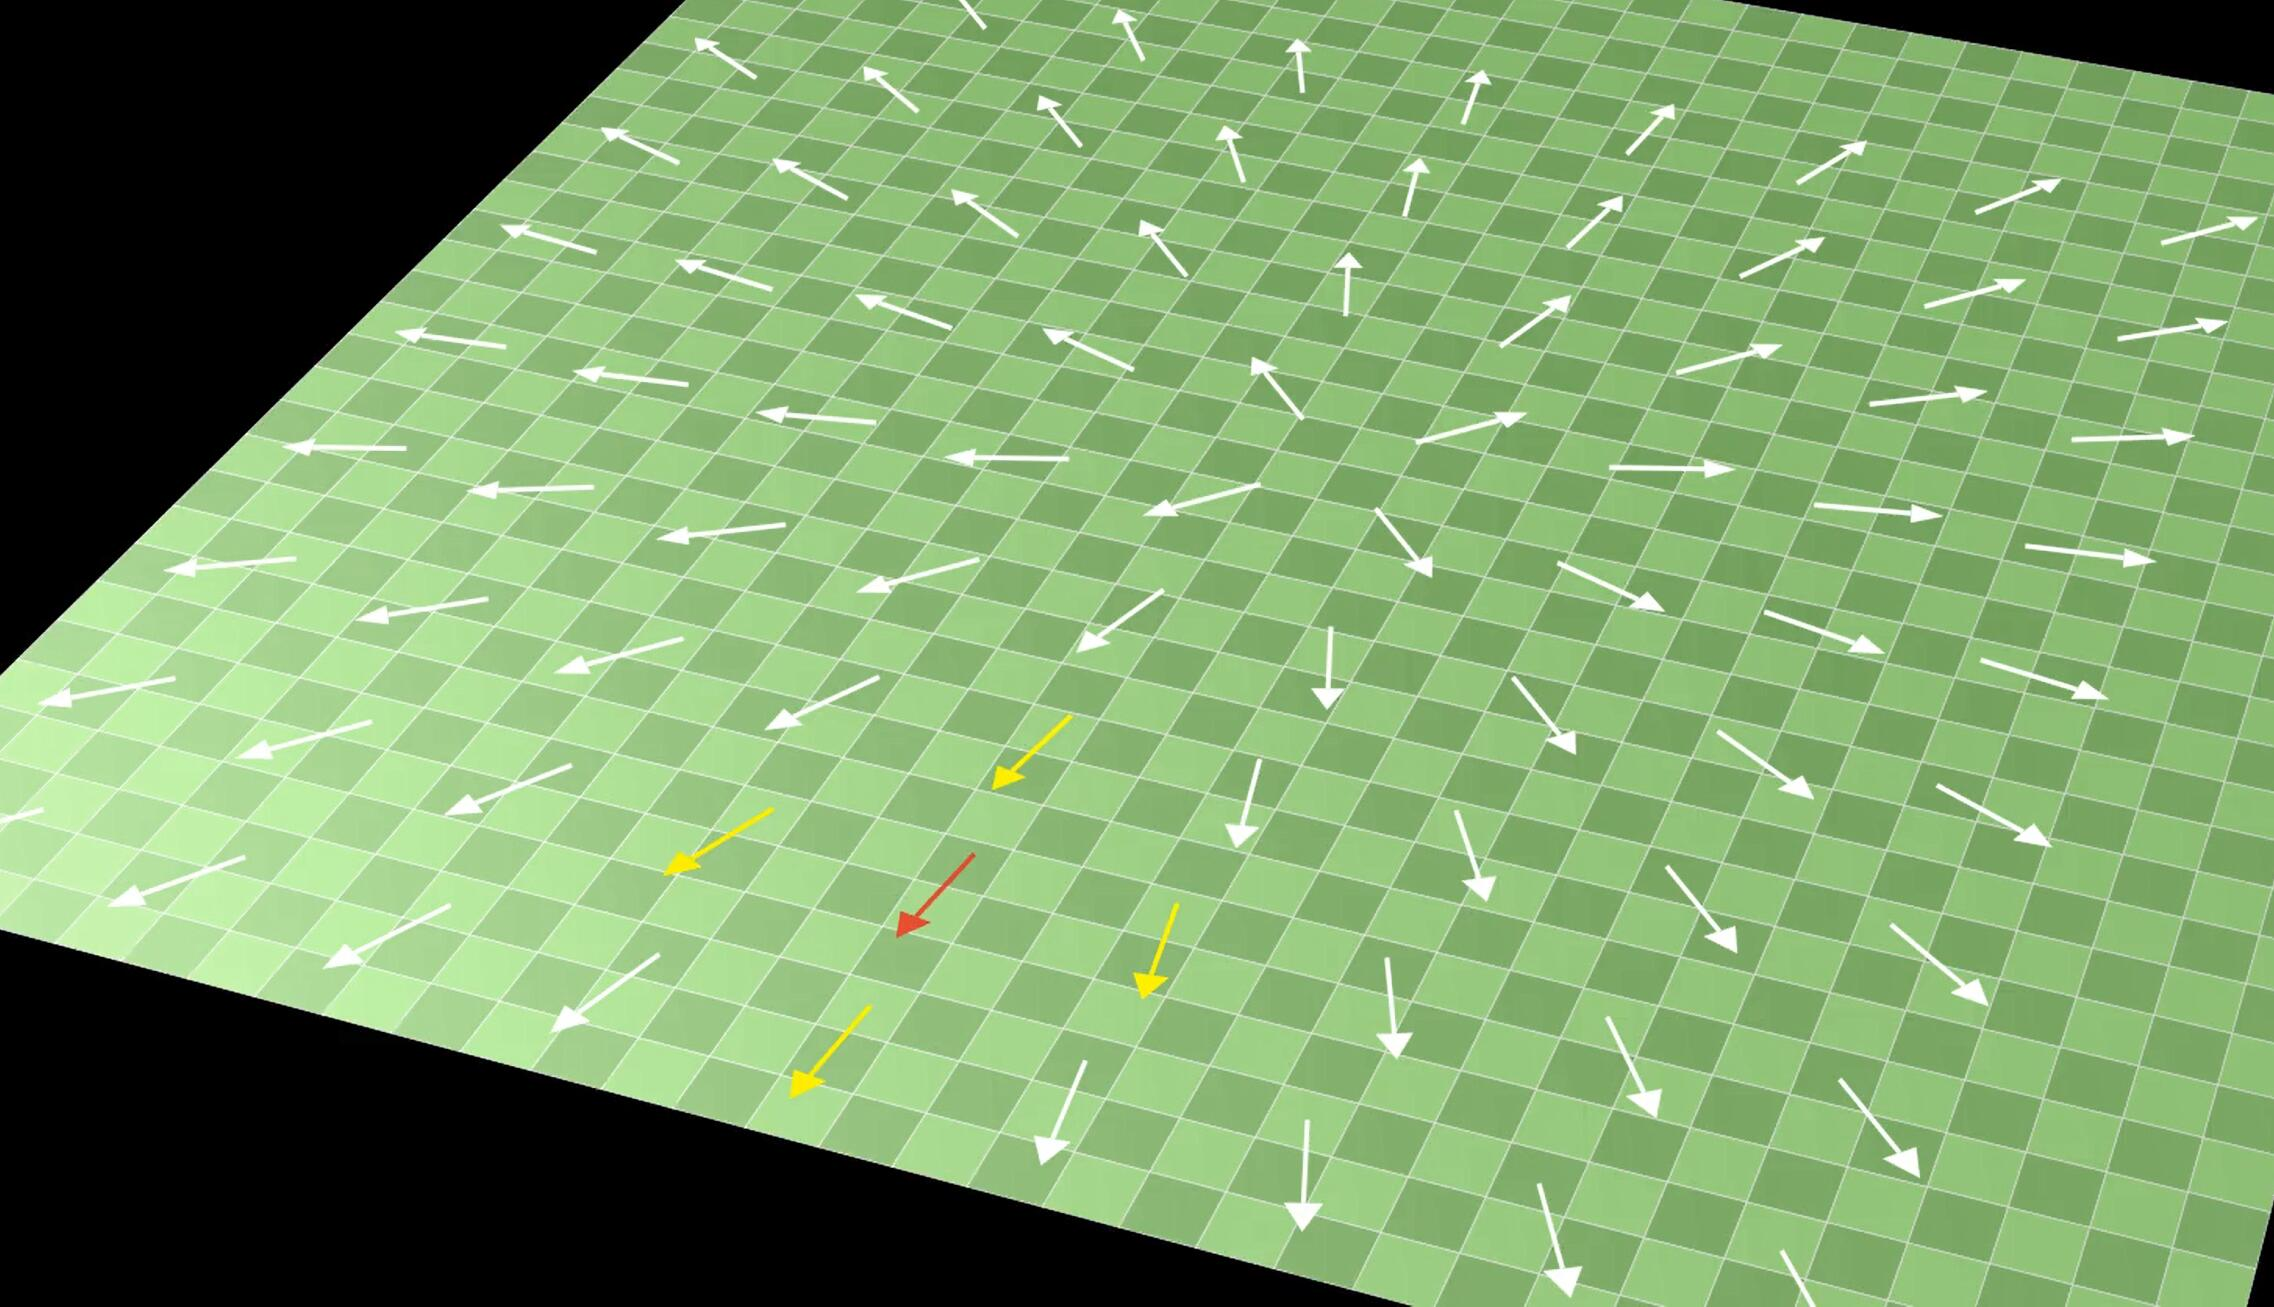
\includegraphics[width=.45\linewidth]{fig/flat}} \quad
%   \subfloat[Manifold with geodesic metric distance D(q,k) changed, causing neighbour change.]
%   {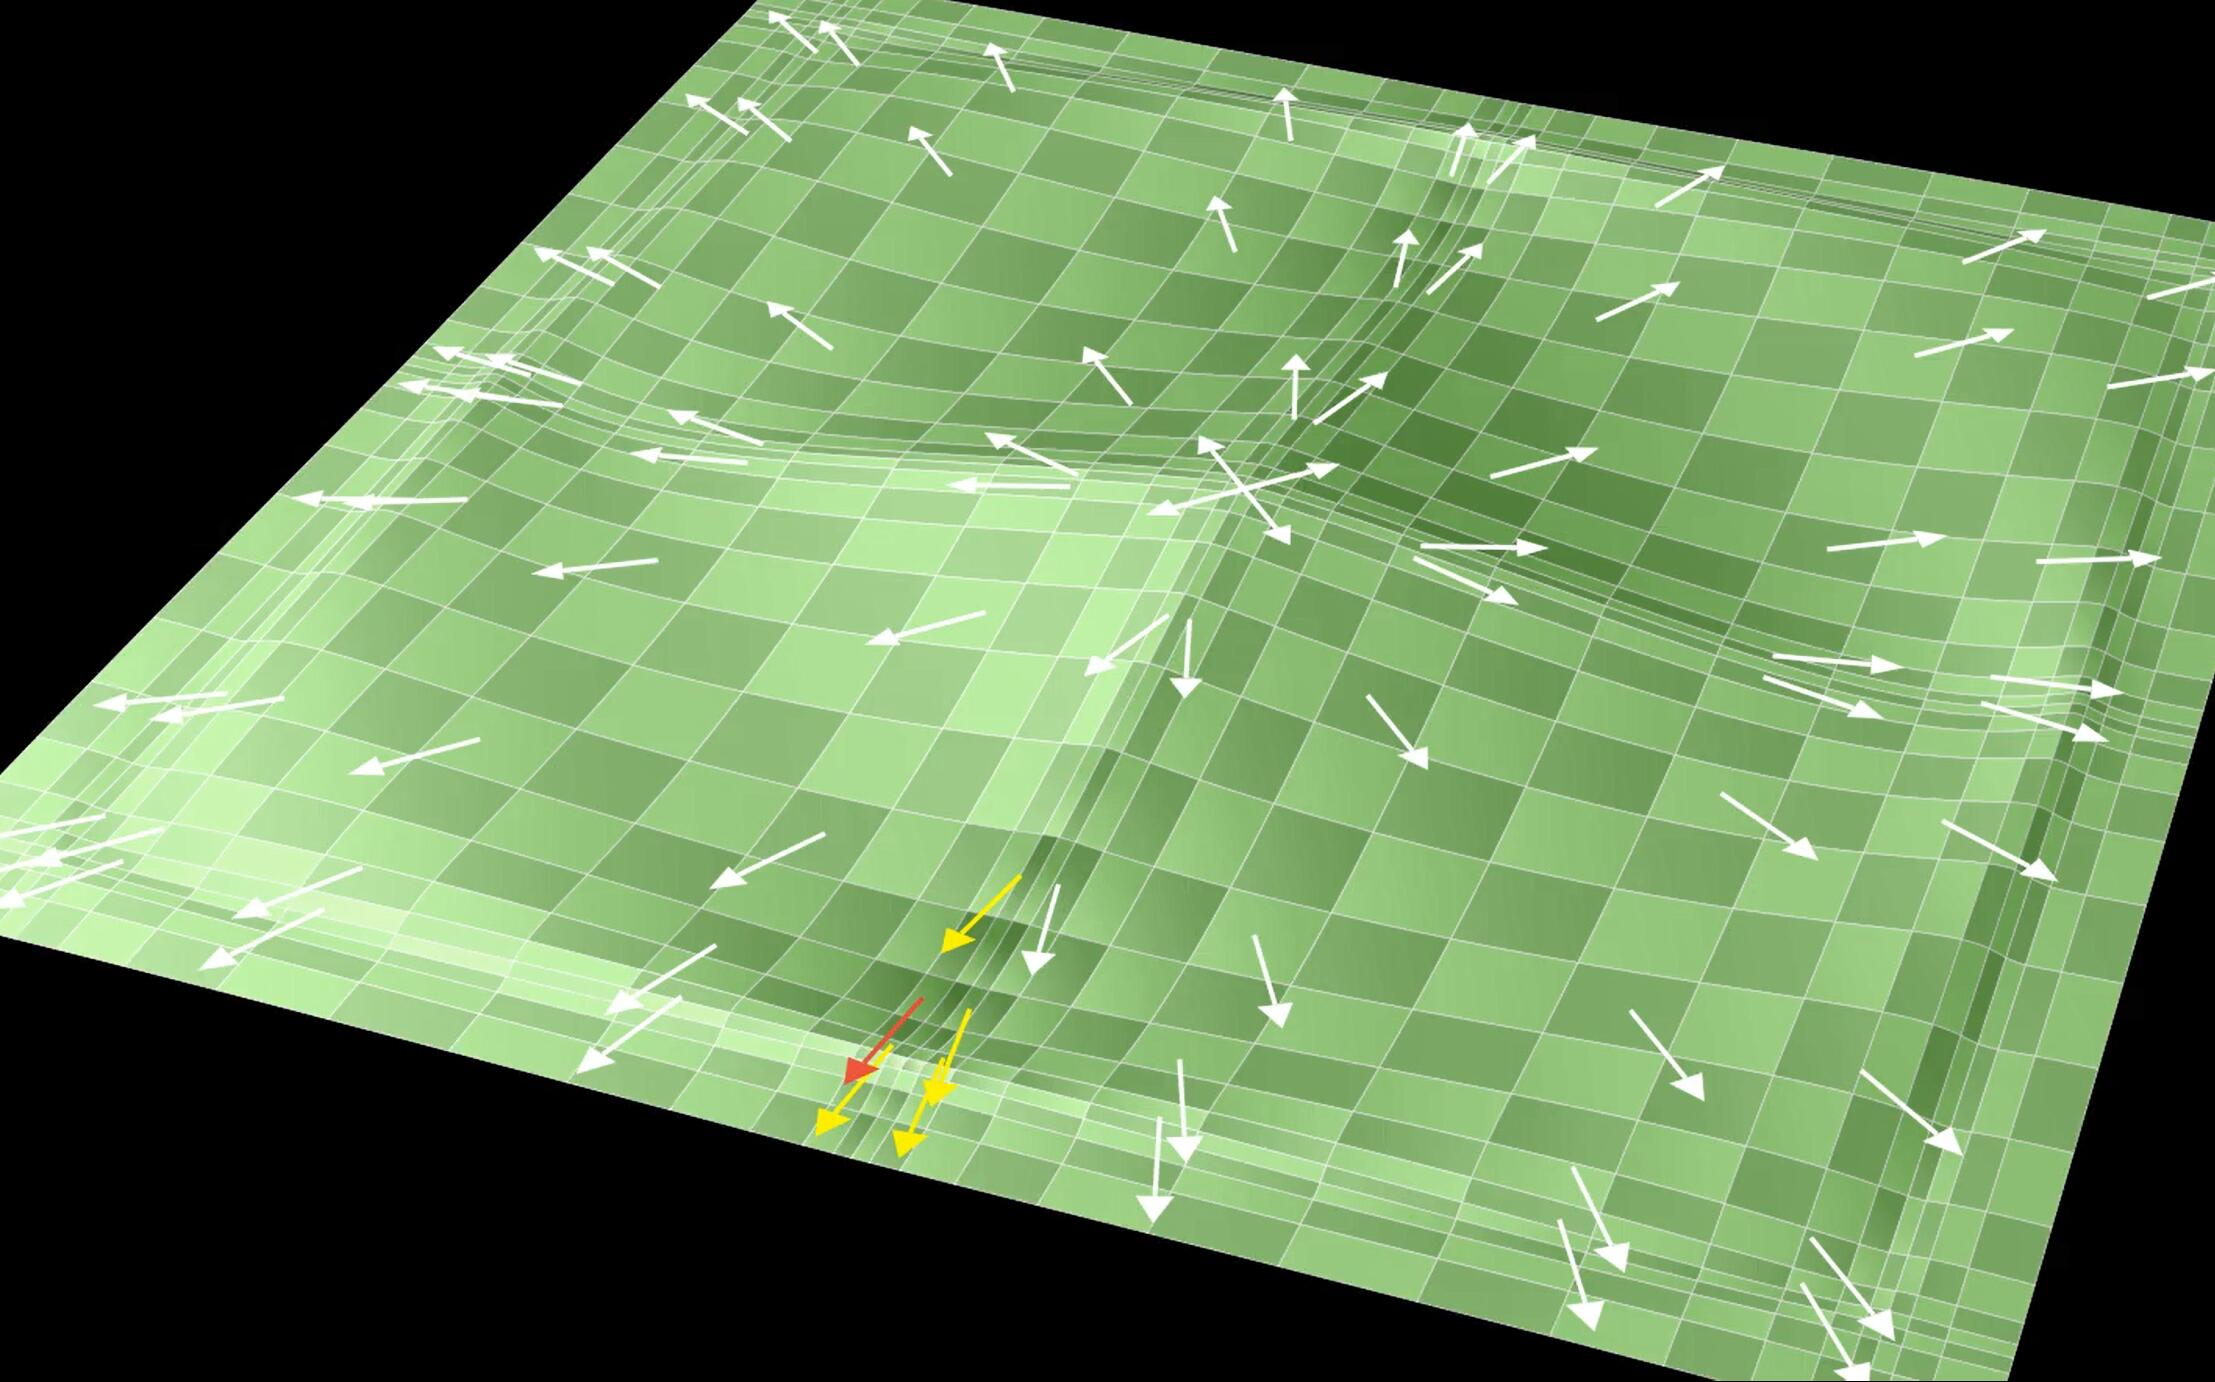
\includegraphics[width=.45\linewidth]{fig/manifold}} \quad
%   \subfloat[Attended value(orange) is differ from the original value(red)]
%   {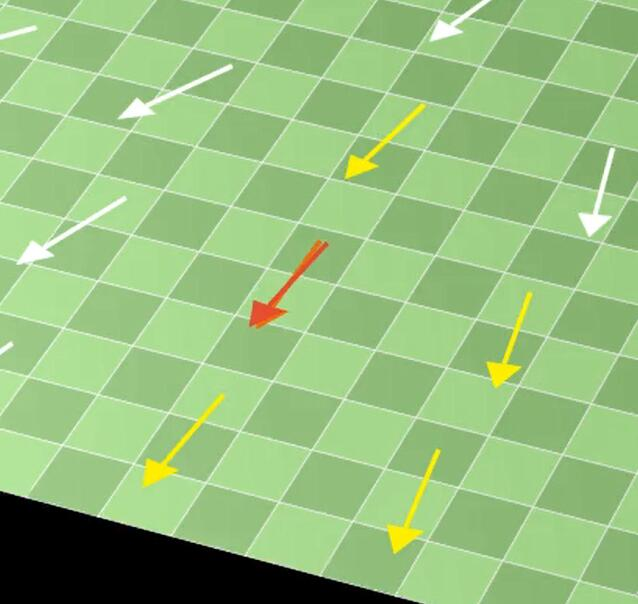
\includegraphics[width=.45\linewidth]{fig/diff}} \quad
%   \subfloat[zoomed in to show difference]
%   {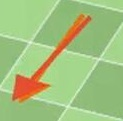
\includegraphics[width=.45\linewidth]{fig/diff2}} \quad
%   \caption[geometric interpretation of parametric self-attention]{geometric interpretation of parametric self-attention}
%   \label{fig:attention}
%   \end{figure}


  \subsection{GPT worldlines}
  Take one GPT layer, self-attention transformer receives input signals following different worldline trajectories. Fig\ref{fig:worldlines-gpt} shows $\boldsymbol{x}_1$ signal need to travel at a lower speed compare with $\boldsymbol{x}_2$ speed, if both of them need to arrive transformer at time T. 
  This is also reflected in the gradient of trajectories in space-time diagram. To be more intuitive, assuming travelling speed is constant and path length of signal conduction is extended as a compensate. This describes better towards reality, plotted in the constant speed picture of space-time diagram. 
  Signals travelling from an emitter to a target receiver with a fixed spatial location, it can choose multiple paths, each path has a different length so that the travelling time will be a spectrum of durations. 
  Noticing the route probability is not the same thing as self-attention weight. Self-attention weights are calculated within transformer as receiver at time T, whereas route probability is formed at emision time in the source input neuron position. 
  $\sum\limits_{i} a_{i,T}=1$ is the normalization of self-attention weights, whereas $\sum\limits_{t} \frac{n_{1,t}} {N} = 1$ is the normalization of route probabilities, N is the total number of signals emitted per unit time if neuron $x_1$ is activated. 


  \subsection{Goal as function convolution}
  Method of calculating similarity between two signals is dot product.  
  Query signal is the external magnetic force experienced at target(destination) location, Keys are signals arriving target from different sources. A route is defined as a (source, target, travel\_duration) triplet. 
  Now we implement the same idea of attention weight update on emision route probabilities. If the arriving signals are similar to the target, then increase the corresponding route probability. The consequence would be if we randomly pick two signals arriving at same time in any self-attention event, 
  if they are similar, then source neurons will send more signals along the two paths with correct travelling duration, so that more signals would follow these paths and interact in the same 'meeting' event. 
  If query vector is always present and acting as a host, he can welcoming similar guests to join his meeting and expelling unwanted dissimilar guests since accepting those guests will cost more energy. 
  Define this process as \textbf{magnetic induction mutual attention}. After route probability update is completed, signals arriving an attention interaction 'meeting' will form a \textbf{constructive interference}.  
  
  If signals do not disappear immediately after his arriving 'meeting' event, it may interact with signals arrive in the future. 
  Our assumption is that signals must arrive simultaneously and are not allowed to survive after 1 timestamp, because old meeting event will be dismissed to allow the next meeting to start. 
  The reality may not be so strict. Two signals do not have to arrive simultaneously to enable self-attention interaction; as long as their worldline routes converge into a vacinity range in space-time diagram, 
  self-attention interaction can take place. This situation is ignored for simplicity reason. 
  
  Host signal is assumed to be present all the time. 
  Consider all the guest signals and their arrival time distribution, $\boldsymbol{f}(t) = \int\limits_{\tau = 0}^{t} \rho_{\tau,t} \boldsymbol{x}(\tau) d\tau$ is the resultant signal received by host at time t. $\rho_{\tau,t}$ is the emision number per unit time from source neuron at time $\tau$ and arrives attention interaction event held at time $t$. 
  Our goal is to maximize the peak of similarity between target signal and the received signal $J=\sup_{t \in [0, T]}\boldsymbol{f}(t) \cdot \boldsymbol{g}(t)$. This is the maximum instantaneous energy of the ising model. If the peak is high enough then hopefully the host will be able to emit signals to the next layer or triggers an avalanche of phase change in the ising model. For simplicity, assume the target host signal is
  $$
    \boldsymbol{g}(t) =\left\{
    \begin{array}{rcl}
    \boldsymbol{1} &  & 0 \le t \le T\\
    \boldsymbol{0} &  & \text{otherwise}
    \end{array}
    \right.
  $$
  Host signal is set to be a top-hat function with constant vector same size as signals $\boldsymbol{1}=(1, 1, ..., 1)^T$ during the interaction time period $[0, T]$. 
  Therefore the goal becomes a convolution function, which describes the strength of influence caused by impulse of arriving signals. 
  This is also the peak of energy-over-time function in our simplified ising model.
  $$J=\sup_{t \in [0,T]} \int\limits_{\tau=0}^{t} \rho_{\tau,t} \boldsymbol{x}(\tau) \cdot \boldsymbol{1} d\tau$$

  This goal applies to a single learner which can only response to one class. In order to solve a multi-class classification problem, we will need multiple learners.
\end{multicols}

\begin{figure*}[bth]
  \myfloatalign
  \subfloat[signal worldlines in GPT model]
  {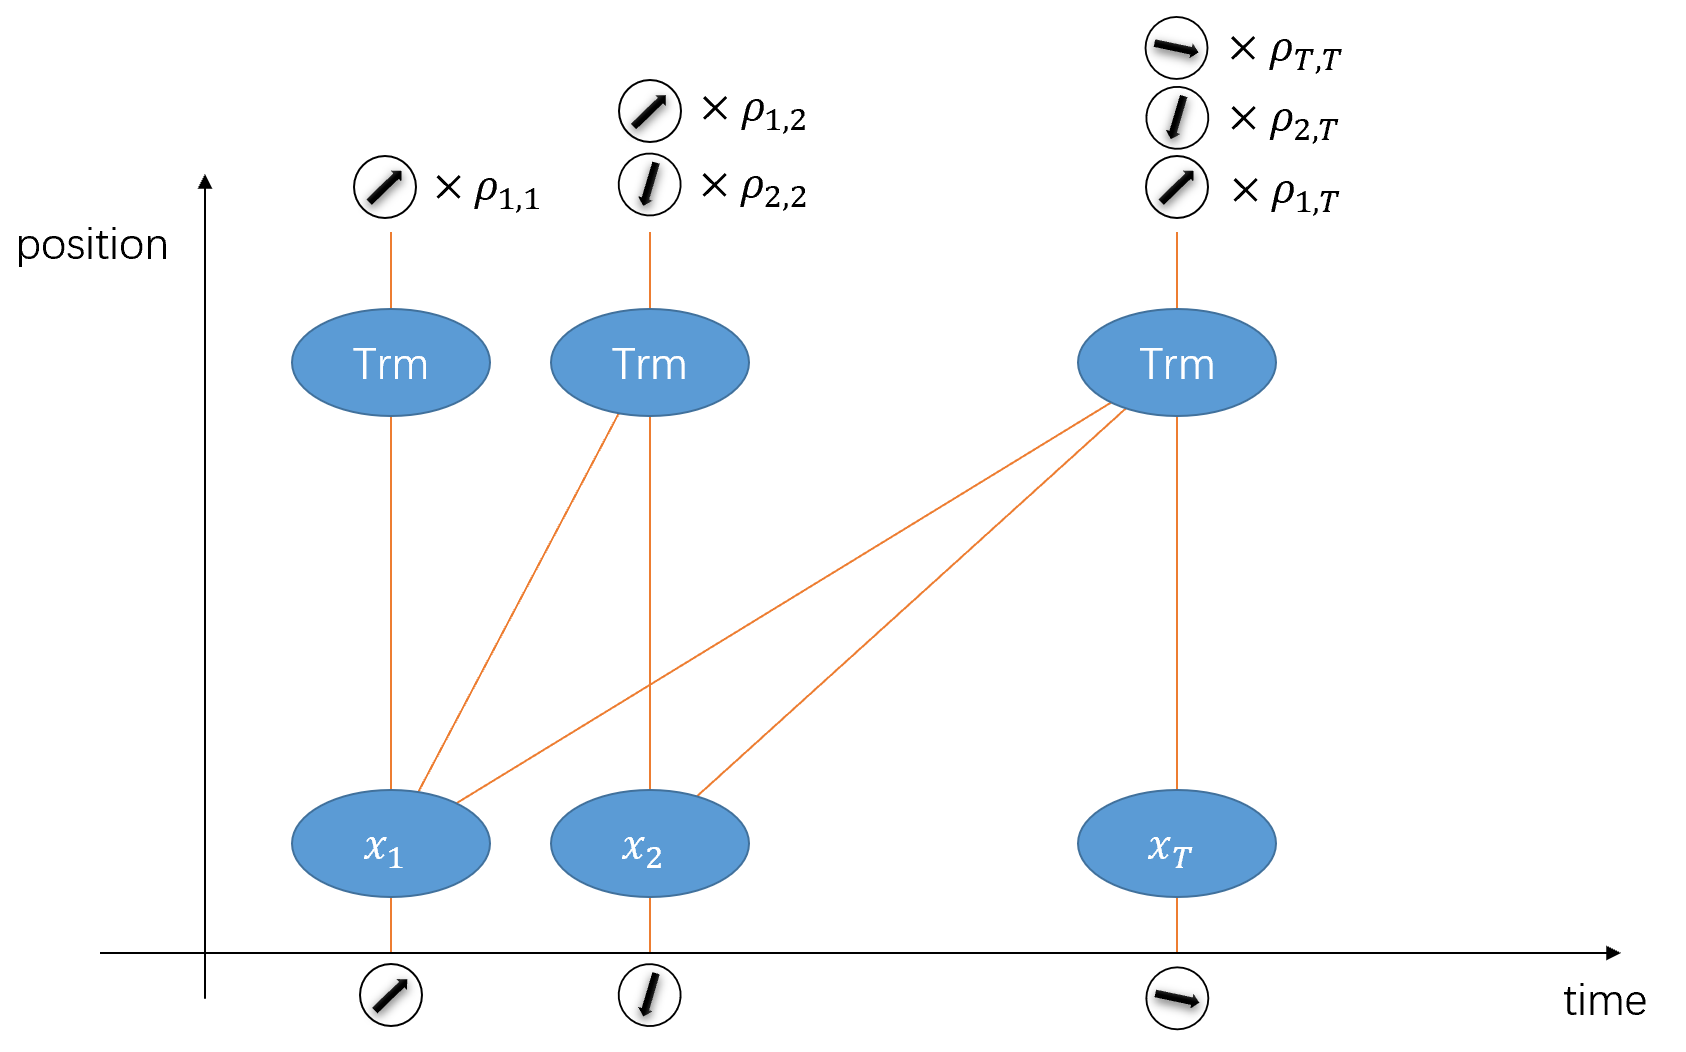
\includegraphics[width=.45\linewidth]{fig/gpt-worldline.png}}
  \subfloat[constant speed worldlines]
  {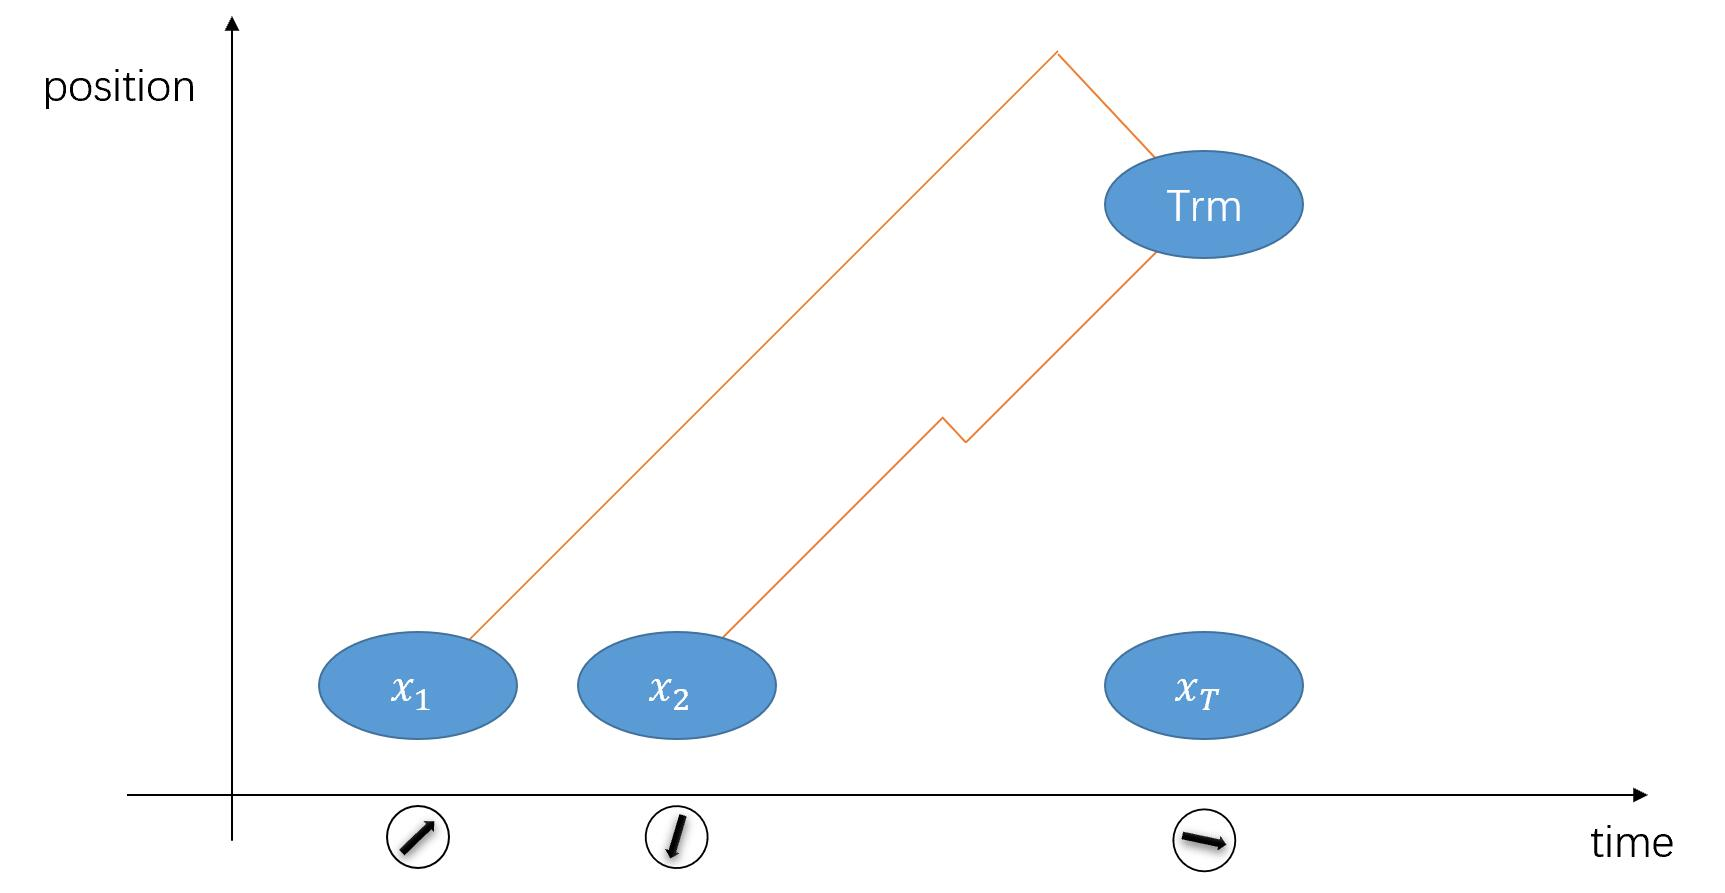
\includegraphics[width=.45\linewidth]{fig/worldline_const_speed.jpg}}
  \caption{space-time diagram of signals} \label{fig:worldlines-gpt}
\end{figure*}

\clearpage
\section{Method}

\begin{figure}
  {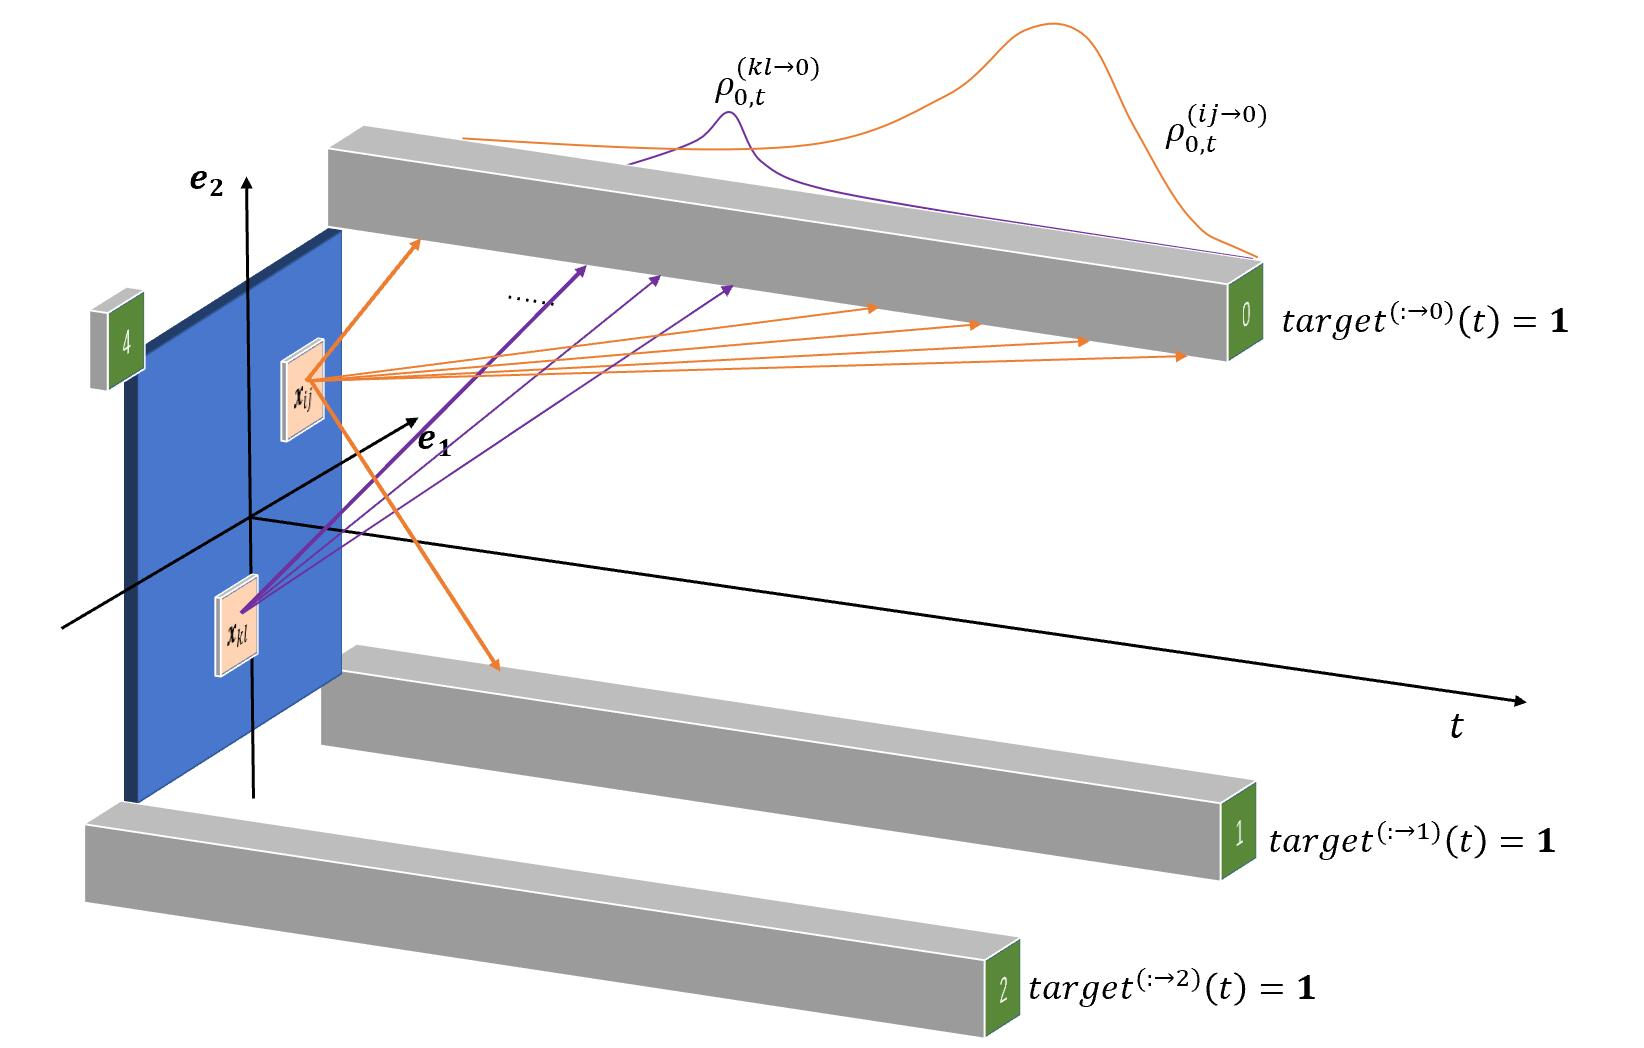
\includegraphics[width=1.0\linewidth]{fig/mnist_spacetime.jpg}}
  \caption[4-class worldlines]{4-class worldlines}\label{fig:mnist-spacetime}
\end{figure}

\begin{multicols}{2}
4 classes are chosen out of 10 from MNIST dataset, $y \in \{0, 1, 2, 4 \}$. Spatial dimention is 2 in order to input features of a 2D picture, plus one temporal dimention to form our space-time diagram.
Preprocessing the picture requires truncation to size [27,27], cutting into non-overlapping 3x3 regions, then reshaped to [W,H,9], where W=9 and H=9. Size of signal vector is 9+1, and there are WxH=81 different sources of signals. 
The extra one size of signal is used to represent the resting state, in case if all the 9 pixels are all 0, the normalized signal can still have modulus length equals to 1. $\boldsymbol{x}_{ij} \cdot \boldsymbol{x}_{ij} = 1 \forall i \in [1, 9], j \in [1, 9]$, $\boldsymbol{x}_{ij} \in \mathbb{R}^{10}$.
 4 target classes are placed just outside the spatial corners of the picture as shown in Fig\ref{fig:mnist-spacetime}. 
Target signal also has its size increased by 1. 
$$target^{(:\rightarrow y)}(t) = \boldsymbol{g}_y = \begin{pmatrix} 0 \\ \frac{1}{3}\boldsymbol{1} \in \mathbb{R}^{9} \end{pmatrix} \forall t \in [0, T]$$
All signals are zero-centralized and then normalized, having modulus length equals 1. Anywhere else in this paper whenever a $\boldsymbol{1}$ appears, it really represents $\boldsymbol{g}_y$, the unattended constant target signal, physically interpreted as the magnetic external field.

Manhattan distance is used to calculate spatial distances, signal speed is set to be constant 1. Every souce ij maintains its own route probability matrix. Time is truncated at T=24, enough for any signal to reach its target destination (maximum distance is 18), 
plus 6 timestamps to receive final signals for the system to reach equilibrium. 
Each route probability matrix has shape [4, 25], covering the 4 corner classes with any travel duration $t-\tau \in [0, 24]$. There are routes not possible of travelling because of the speed limit, and also there are routes detoured so signal would arrive later than expected. 
No noise is add along the routes, and no transformation is applied to the travelling signals. 

Each training step, only one input picture is fed into the network, allowing system to evolve 24 timestamps, apply attention mechanism at each timestamp interaction event, meanwhile accumulating the modification on each travelling duration. After 24 timestamps the accumulated modification is applied to the route probabilities and then normalized. 

Mutual attention is applied between target host as query and input signals as keys to obtain the attended target:
$$
\boldsymbol{h}_{y}(t)=\sum\limits_{m(t)} \frac {s_{ym}} {\sum\limits_{l',m'} s_{l'm'}} \boldsymbol{v}_{m}
$$
where 
\begin{equation}
s_{ym} = \left \{ 
\begin{array}{rcl}
1 & & \text{if } \boldsymbol{q_y}\cdot\boldsymbol{k_m} \ge 0.7 \\
0 & & \text{elsewise}
\end{array}
\right .
\label{threashold-attn}
\end{equation}
This is just averaging the query with all keys having similarity greater than a threashold, under the constraint that signal could arrive the target location in time.  
$\boldsymbol{k}_m = \boldsymbol{x}_{ij}(\tau)$ with source id $m(t):=9i+j \mid dist(ij\rightarrow y) \le t-\tau$; and query $\boldsymbol{q}_y=\boldsymbol{g}_y = \boldsymbol{1}$.

After attention, target with all similar neighbours would have similarity equals 1, and the remaining signals would interact with the attended host target in the convolution: 
\begin{equation}
\begin{split}
J_y=\sup_{t \in [0,T]} \int\limits_{\tau=0}^{t} \sum\limits_{ij \mid s_{ym}=0}\rho_{\tau,t}^{(ij \rightarrow y)} \boldsymbol{x}_{ij}(\tau) \cdot \boldsymbol{h}_y(t) + \\
 \sum\limits_{ij \mid s_{ym}=1} \rho_{\tau,t}^{(ij \rightarrow y)} 1 d\tau
\end{split}
 \label{loss_eq}
\end{equation}

The goal is not maximised using gradients and back propagation. Instead we want to deliver all signals emitted from any source to the correct path, i.e. 
$\rho_{\tau,t}^{(ij \rightarrow y)} = N p_{\delta}^{(ij \rightarrow y)}$, The duration of travelling is $\delta=t-\tau$, N is the total number of signals emitted per unit time in one exitation period from source neuron ij towards target y, which can be treated as constant. 
As route probability $p_{\delta^*}^{(ij \rightarrow y)} \rightarrow 1$, with a suitable choice of travel duration $\delta^*$ on each source-destination combination (i,j,y), a signal can interact with as many similar ($\ge 0.7$ threashold) 'friends' as possible, hence after the attention process, 
$$J_y \rightarrow \sum\limits_{ij \mid s_{ym}=1} \int\limits_{\tau=\tau_{emit}}^{t^*(i,j,y)=\tau_{emit}+\delta^*} N d\tau$$
because the first dot product term in Eq\ref{loss_eq} goes to 0 due to conservation of probability.

This implies if our goal is to minimise the infimum of negative potential energy (as an alternative way of saying maximising $J$), all \textbf{similar} signals chosen by host shall arrive at $t^*(y)=t^*(i,j,y) \forall i,j$ simultaneously, forming a sharpe spike on graph showing received signal number distribution over time, producing a low entropy state. 
Due to the presence of host signal $\boldsymbol{g}_y(t)$, generalized to be time dependent, $t^*(y)$ is expected to appear around the peak of $\boldsymbol{g}_y(t)$'s magnitude. 

$$
\rho^{:\rightarrow y}(\tau, t) = \sum\limits_{ij} \rho_{\tau, t}^{ij \rightarrow y}
$$
In the MNIST experiment signals are emitted only at $\tau=0$, therefore for target y, the similar signals' entropy is 
$$H_y=-\int\limits_{t=0}^T q(t) log q(t) dt$$ 
where $q(t) := \frac{\rho^{+\rightarrow y}(t)} {\int\limits_{t=0}^T \rho^{+\rightarrow y}(t) dt}$ and the superscript symbol '+' means all the similar signal sources. 
This entropy is expected to decrease in order for the similar signals to induce a larger power. 

However under the assumption that target external field is time-independent rather than a spiky impulse, the updating rule we are using is optimizing the energy during all time, 
not trying to concentrate the receiving peak, so there is a slight mismatch between our goal and the weight updating rule. Despite this difference the model can still learn, more detailed analysis will be done in the Experiment section. 

Route probability update method is simple, adding a modification term and then re-normalize over travel duration $\delta = t-\tau$: 
\begin{equation}
  p_{\delta}^{ij\rightarrow y}(new) = \frac{ p_{\delta}^{ij\rightarrow y} + \Delta w_{\delta}^{ij\rightarrow y}} {\int\limits_{\delta} p_{\delta}^{ij\rightarrow y} + \Delta w_{\delta}^{ij\rightarrow y} d\delta }
  \label{eq:update-rule}
\end{equation}
$$
  \Delta w_{\delta}^{ij\rightarrow y} = \left \{
  \begin{array}{rcl}
    \eta_{+} p_{\delta}^{ij\rightarrow y} & & \text{if } \boldsymbol{x}_{ij} \cdot \boldsymbol{g}_y \ge 0.7 \\
    \eta_{-} p_{\delta}^{ij\rightarrow y} & & \text{if } 0.7 > \boldsymbol{x}_{ij} \cdot \boldsymbol{g}_y > -0.7 \\
    \eta_{--} p_{\delta}^{ij\rightarrow y} & & \text{if } \boldsymbol{x}_{ij} \cdot \boldsymbol{g}_y \le -0.7
  \end{array} \right .
$$
where $\eta_{+}$, $\eta_{-}$, $\eta_{--}$ are learning rates for different similarities between arriving signals and target. 
Learning rates can vary for different number of training samples. For C=4, K=5 few-shot setup, $\eta_{+}=1.0$, $\eta_{-}=-0.5$, $\eta_{--}=-0.8$ are chosen. 
0.7 is a threashold defining the term 'similar', which can also be changed.

After the model is trained for 1 epoch, inference process is to calculate $J_y$ according to Eq\ref{loss_eq} $\forall y \in \{\text{label set}\}$ as if they are activated, the prediction is $y_{pred} = \mathop{\arg\max}_{y}  J_y$ 

\end{multicols}

\section{Experiment}

\begin{table*}[]
  \centering
  \begin{tabular}{|l|l|l|l|l|}
  \hline
             & \begin{tabular}[c]{@{}l@{}}C=4,K=1\\ epoch=5\end{tabular} & \begin{tabular}[c]{@{}l@{}}C=4,K=5,\\ epoch=1\end{tabular} & \begin{tabular}[c]{@{}l@{}}C=4,K=10\\ epoch=1\end{tabular} & \begin{tabular}[c]{@{}l@{}}C=4,K=5\\ epoch=10\end{tabular} \\ \hline
  Our+SeqTrn & 66.63\%                                                   & 83.50\%                                                    & 88.65\%                                                    & 86.99\%                                                    \\ \hline
  Our+MixTrn & NA                                                        & 86.66\%                                                    & 82.48\%                                                    & 83.81\%                                                    \\ \hline
  BP+SeqTrn  & 38.41\%                                                   & 43.79\%                                                    & 35.04\%                                                    & 77.23\%                                                    \\ \hline
  BP+MixTrn  & NA                                                        & 53.28\%                                                    & 53.86\%                                                    & 79.99\%                                                    \\ \hline
  \end{tabular}
  \caption {few-shot experiment results}
  \label{tab:ck-results}
  \end{table*}
\begin{multicols}{2}
  \subsection{MNIST classification}

  Few training examples are randomly selected from MNIST, forming 3 train sets, each contain 1, 5, 10 pictures per class respectively. 
  One picture is fed into the network for each train step. Sequential train receives inputs from different classes in sequential order; mixed train shuffles the input order. 
  For example with [a,b] being the two classes, SeqTrn(C=2,K=3)=[a,a,a,b,b,b], whereas MixTrn(C=2,K=3)=[a,b,b,a,b,a]. 
  A number of epoch repeats the train procedure. 

  A fully connected neuron network with self-attention appled on input layer, then through a fully connected trainable weights of shape [4, 729], 
  predicting a softmax probability, using cross-entropy loss and Adam optimizer to back propagate the gradients. This one-layer model is the usual way of training, 
  and it is the compare benchmark for our proposed induced interference training.

  Test is evaluated on MNIST test set only using the 4 training digits [0,1,2,4]. 


  Our dynamic induced interference training outperforms the traditional back propagation model in few-shot scenario, 
  and it doesn't suffer from the catastrophic forgetting in sequential training. Result is in Table\ref{tab:ck-results}. In fact sequential learning can sometimes be more hepful. 
  For the one-shot situation, mixed training makes no difference with sequential training, but the accuracies are largelly influenced by the quality of the one chosen picture. 
  Therefore the one-shot experiments are repeated for several times and then take the average accuracy. 
  Increasing K and epoch number can eventually let the BP network to achieve accuracies up to 94\% or higher, but clearly human learning doesn't require that much data and train steps. 
  
  Catastrophc forgetting is another important effect need to be addressed. Classical fully connect matrix transforms the common manifold where all input signals are projected on. 
  Learning one class will affect the shape of manifold and hence the relative distances between current input vector forwarded onto the hidden layer and the anchor vectors ($\boldsymbol{W}[y,:] \forall y \neq target$) of other classes, 
  therefore changing the output similarity with other classes. 

  In our ising model based forward propagate mechanism, route probabilities towards different target learners are normalized separately, 
  updating the probabilities towards $y=0$ doesn't affect the $y=1$ routes, therefore forgetting is not obvious, unless most of the two different class's input sources cannot distinguish the two target's space-time coordinates. 
  This circumstance is like employees adjusted their departure time to arrive their working company at 9:30 am normally; 
  then the next day their working place is moved to another venue,  
  all the employees leave home as usual time and still arrives the new company venue around a same time; this is highly unlikely to happen without the employees re-adjust their departure time. 

  If the similar signals cannot arrive simultaneously, then the proportion of dissimilar signals in an attention event will increase. 
  This will cause the expected similarity between any two signals to decrease. This effect has been proven; diagonal along Table\ref{tab:similar} 
  has shown the estimated similarity metric after training has finished, and the supervising external target signal field has been withdrawn for this evaluation. 
  In a learner's receiver view, probability distribution of arriving signal count over all sources can be calculated. This probability distribution becomes stable as more signals 
  are arriving towards the end of observing time window. 18 timestamps is the lower bound of travelling time for the furthest separated source-destination pair. 
  This leaves 6 timestamps corresponding to 6 snapshots of complete-information interaction events, calling this the sable period. 
  Therefore each snapshot the expected similarity can be calculated as:
  $$
  \mathbb{E}_{q_l, q_m} S(t) = \sum\limits_{lm} q_l q_m \boldsymbol{x}_l \cdot \boldsymbol{x}_m
  $$
  where $l \in \{1...81\}$ loopping through source ids, and probability of receiving a signal from the source is
  \begin{equation}
  \begin{split}
  q_{l}(t) = \frac {\int\limits_{\tau}^t\rho_{\tau,t}^{i,j\rightarrow y} d\tau} {\sum\limits_{l} \int\limits_{\tau}^t \rho_{\tau,t}^{i,j\rightarrow y} d\tau} \\ 
  \forall l=9i+j
  \end{split}
  \end{equation}

  Then the expected similarity is averaged over $t \in [19,24]$ for a number of input examples selected from a desired label. 
  4 learners all have a largest expected similarity for their own label. This is a solid evidence that the inducing external field's precense 
  during training process is helping the input signals to show greater expected similarity only in the correct learner. 
  This is the same analogy as magnitizing a neutral iron block using a magnant. Take away the magnant, the iron block still exhibit magnetic field only in certain direction.

  Another interesting phenomenon was observed when analysing the expected signal arrival time shown by Table\ref{tab:arrival-time}. 
  We know the sources are sending signals with different travelling durations according to a distribution. A distribution is trained for each 
  target destination, so there are 4 trained signal sending policies, making up the route probability array. What would be the consequence of using a 
  wrong policy on any target? Obviously the optimizing objective would not be as high as if the correct policy is used because constructive interference would be broken. 
  Apart from that, according to experiment, when white input is used, all sources send signals at same time, 
  the expected signal arriving time using a wrong policy would be shorter than the time if the correct policy is used. 
  Although is is not always true if learners are re-trained, but most of the time this effect has been observed. 
  It seems to suggest that in human thought, correct answer usually takes longer time to be realized, and the first impression answer is likely to be wrong. 
\end{multicols}

\begin{table*}[]
  \centering
  \begin{tabular}{|l|l|l|l|l|}
  \hline
           & y=0    & y=1    & y=2    & y=4    \\ \hline
  learner0 & 0.2971 & 0.1876 & 0.0914 & 0.1559 \\ \hline
  learner1 & 0.1551 & 0.4441 & 0.1507 & 0.1130 \\ \hline
  learner2 & 0.0833 & 0.1168 & 0.1912 & 0.0534 \\ \hline
  learner4 & 0.0951 & 0.1608 & 0.1258 & 0.2409 \\ \hline
  \end{tabular}
  \caption{expected signal similarity during stable period} \label{tab:similar}
  \end{table*}

\begin{table*}[]
    \centering
    \begin{tabular}{|l|l|l|l|l|}
    \hline
              & policy0 & policy1 & policy2 & policy4 \\ \hline
    learner0 & 15.99   & 9.49    & 10.17   & 7.24    \\ \hline
    learner1 & 18.05   & 18.49   & 13.63   & 12.75   \\ \hline
    learner2 & 17.24   & 14.28   & 17.97   & 17.51   \\ \hline
    learner4 & 9.72    & 10.31   & 9.89    & 15.43   \\ \hline
    \end{tabular}
    \caption{expected signal arrival time for sending policy} \label{tab:arrival-time}  
  \end{table*}

\clearpage 
\begin{multicols}{2}
  \subsection{Double slit experiment}
  With signal emision time spanning for a duration $L$, an experiment was firstly designed on a NLP task. 
  However the NLP experiment was not successiful. The main reason of failure is that no activation state can be easily defined for the input word vectors; i.e. 
  $\boldsymbol{wv} \cdot \boldsymbol{1} \neq similarity(word, target)$. Unlike the previous mnist experiment, where the 3x3 feature's activation level can be easily defined, 
  NLP word vectors has been transformed into a number of 'topics' equals to the number of vector size. Each 'topic' has a scalar 'magnitude' but its range cannot simply be stretched to $[-1, +1]$. 
  A viable representation is to use the crude one-hot representation as input, with size of dictionary equals the number of sources, each having a unique position. 
  This would produce a route probability tensor with shape $[N_{dict}, C, T]$, with dictionary size $N_{dict}$, number of classes C and travel duration with maximum value T. This is too large to be trained in practical; 
  for large picture/video inputs this can also be a huge problem for the training.
  Therefore some kind of aggregation+pooling method need to be used in order to reduce the number of signal travelling routes. Such a method will be proposed in the Further Work section. 

  In order to verify whether our induction model works for a time-varying signal source, A double slit experiment was designed to solve a 2-class classification problem. 
  The model was setup to identify whether two signal sources are in phase or out of phase, as shown in Fig \ref{fig:double-slit}. Two signal sources are rotating 2D unit vectors: 
  $$
  \boldsymbol{x}_{i}(t) = \left(
  \begin{array}{rcl}
  sin(\omega t + \theta_i + \epsilon)\\
  cos(\omega t + \theta_i + \epsilon)
  \end{array}
  \right)
  $$
  For the in-phase input, $\theta_0=\theta_1=0$; for the out-of-phase input, $\theta_0=0, \theta_1=\pi$. $\epsilon$ is a small random noise, $\omega$ is the coherent angular velocity of signal rotation. 
  Two targets are both unit vectors $\boldsymbol{y}=(0, 1)^T:=\boldsymbol{1}$. Similar as in the mnist experiment, one dummy dimension is added to represent the 'rest state'. Also the attended target $\boldsymbol{h}_y(t)$ is used to calculate the ising model energy.  

  The idea of the experiment is that if in-phase signals are emitted from input sources, then the route probabilities towards $\boldsymbol{1}^{(0)}$ are trained such that all signals arrived will form a constructive interference pattern at position of $\boldsymbol{1}^{(0)}$. 
  However this doesn't guarenteen a constructive interference in $\boldsymbol{1}^{(\pi)}$'s position with a different route probability policy when input signals remain in-phase. 
  Therefore both the energy averaged over time and the expectation of similarity will be the largest at $\boldsymbol{1}^{(0)}$'s position. 

  The opposite situation occures for the out-of-phase class. Therefore the two learners would be able to solve the classification problem. 

  Experiment shows expected results, model can make predictions with 97\% accuracy.
  The code for both experiments is released. \footnote{https://github.com/ttssrr423/InducedInterference}
\end{multicols}

\begin{figure*}
  {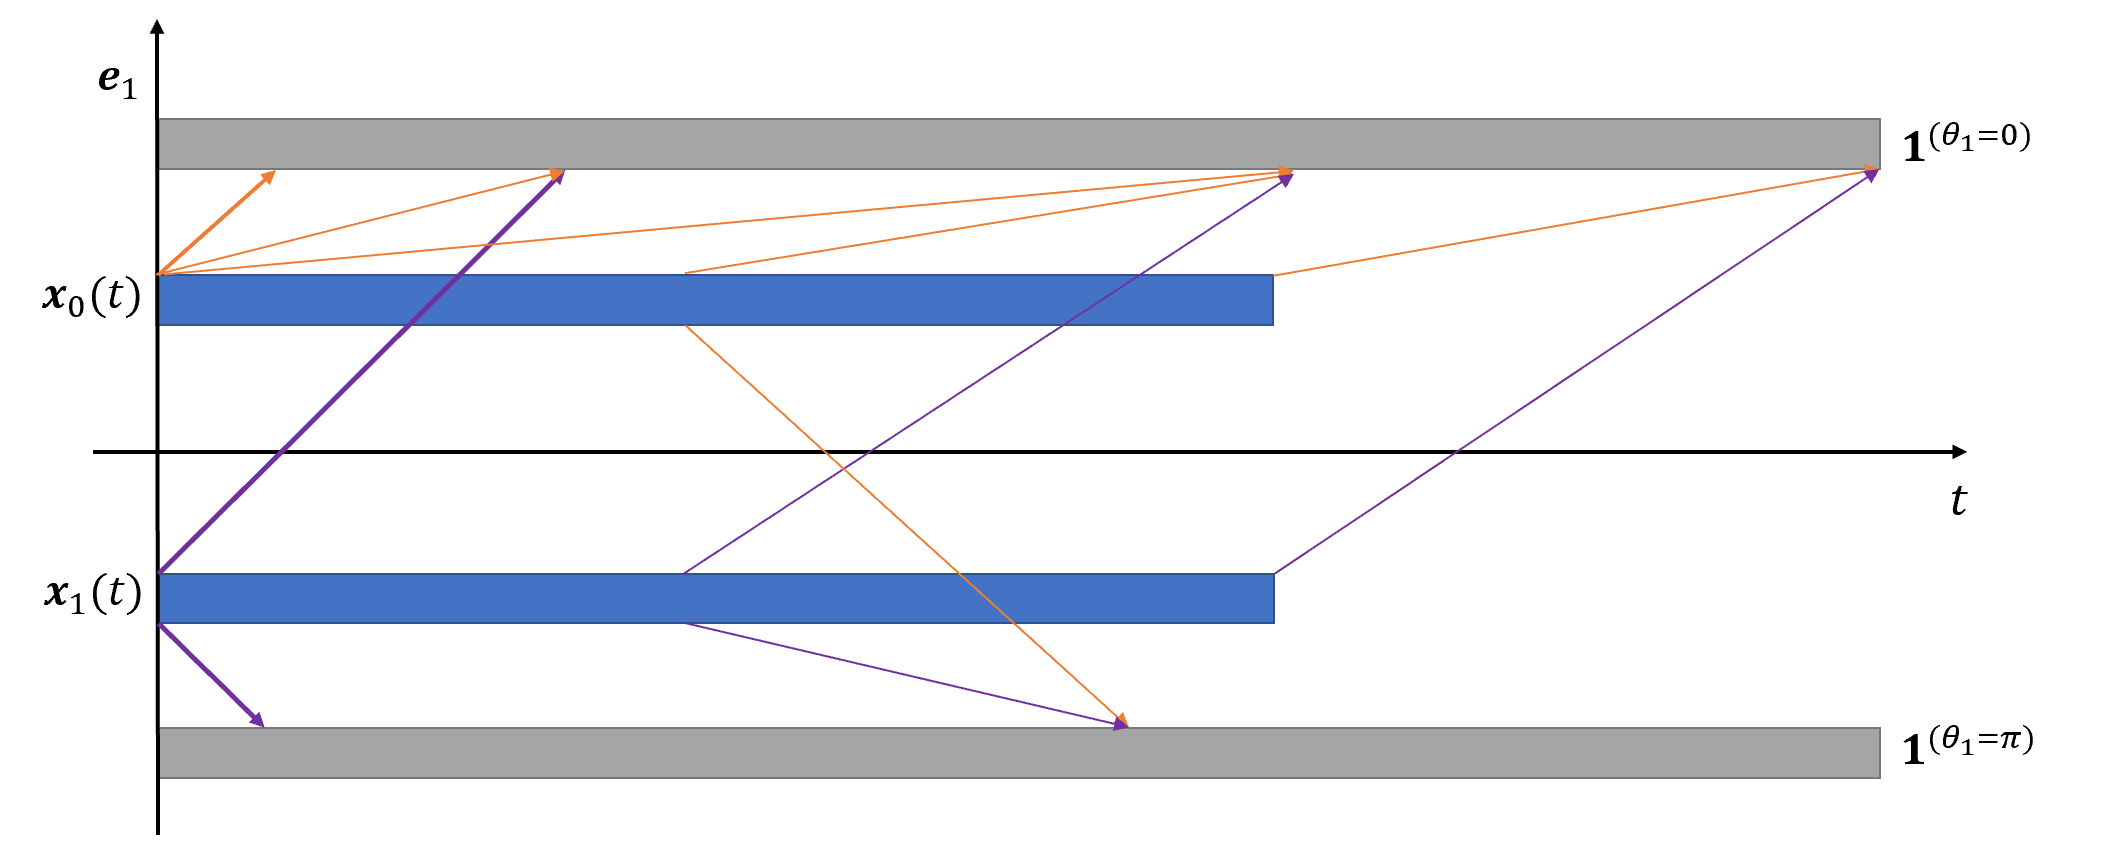
\includegraphics[width=1.0\linewidth]{fig/double-slit.png}}
  \caption{double slit classification}\label{fig:double-slit}
\end{figure*}

\clearpage
\section{Further Work}
\begin{multicols}{2}
  \subsection{Multi-layer encoder}

  There are three things mentioned in earlier section which are not resolved. 
  \begin{enumerate}[]
    \item Dipole-dipole or guest-guest interaction among the arriving signals was ignored. This is an over-simplification.
    \item A method of aggregation+pooling need to be used to reduce the effective number of input sources. This reduces the number of routes need to be trained. 
    \item Non-linearity need to appear somewhere with a reasonable origination. 
    \end{enumerate}
  
  A hierachial attention mechanism is a proposed solution to the problems above. 
  Attention is normally used among vectors, however it can be generalized to be used among any ranked tensors. 
  Scalar attention $h_i=\sum\limits_{j} a_{ij} v_j$ is just perceptron model in another form, with scalar attention weight $a_{ij}(q_i, k_j)$ looked up from a trainable matrix. 
  An vector $\boldsymbol{v}_j^{(1)}$ with elements selected from set $H^{(0)}=\{h_1, h_2,...h_i,...\}$,  forms a subset $\boldsymbol{v}_{j'}^{(1)}=(h_1, h_2, ... h_D) \subset H^{(0)}$. Superscript (1) indicates the rank is 1, therefore a vector is aggregated from rank 0 scalars. 
  Now building the attention mechanism iteratively:

  $$
  \boldsymbol{h}_{i'}^{(1)} = \sum\limits_{j'} a^{(1)}(\boldsymbol{q}_{i'}^{(1)}, \boldsymbol{k}_{j'}^{(1)}) \boldsymbol{v}_{j'}^{(1)}
  $$
  $$
  =\sum\limits_{j'} a^{(1)}(\boldsymbol{q}_{i'}^{(1)}, \boldsymbol{k}_{j'}^{(1)}) \displaystyle\mathop{AGG}\limits_{j'\leftarrow \{i\}} \sum\limits_{j} a^{(0)}(q_i^{(0)}, k_j^{(0)}) v_j^{(0)}
  $$
  
  Superscript on attention weights are indicating the rank of tensor input pairs for the attention similarity function. 
  This equation is the general form of self-attention normally been used. 

  Repeat the aggregation-iteration a few more steps further, a rank R tensor can be treated as the output of the hierachial attention:
  $$
  \boldsymbol{h}_{i'}^{(R)} = \sum\limits_{j'} a^{(R)}(\boldsymbol{q}_{i'}^{(R)}, \boldsymbol{k}_{j'}^{(R)}) \displaystyle\mathop{AGG}\limits_{j'\leftarrow \{i\}} \boldsymbol{h}_i^{(R-1)}
  $$

  Dipole-dipole interactions are allowed to take place among the values in each ranked layer, using a threashold-based attention mechanism as Eq\ref{threashold-attn}. 
  Hence the previously ignored interaction is taken into consideration in a hierachial way. 

  The number of elements in $\boldsymbol{h}_{i'}^{(R)}$ is $D^R$ where D is the number of r-1 ranked tensor in a r ranked tensor. This exponentially increasing size will slow the computation until the forward propagate calculation becomes impossible. 

  The solution to the problem is to use mean-field approximation as the pooling method. In a high rank tensor this enables the dipole-dipole interaction to be modelled. 
  Approximation averages the attended values to produce a scalar, $\mu(\boldsymbol{h}_{i'}^{(R)}) = h_{i'}^{(R \rightarrow 0)}$. A useful property is that similarity between attended value $\boldsymbol{h}_{i'}^{(R)}$ and activation state $\boldsymbol{1}^{(R)}$ now can be calculated using a dot product operation, 
  because more activated elements/neurons will increase their parent tensor's mean field until it reaches the fully activated state $\mu(\boldsymbol{1^{(R)}})=1$. 
  The suqshing of a tensor into a scalar used the idea of renormalization, which can be applied to a complex system not far from its critical state where self-similarity can be observed between different scales.

  Nested concepts with higher level of abstraction represented as a higher rank tensor (larger scale), is a much better way to encode words in tensors, compare with the word vector representation in NLP. 
  This not only fixes the problem of training NLP induced interference network (see 4.2 experiment section), but more importantly, gives rise to the non-linear response towards target signal, experienced as an external magnetic field. 
  Mean field operation reduces the number of input signal sources as well as the signal size. This enables the network to maintain fast forward propagate calculation speed even the attention rank level becomes high.

  Mean field solution of ising model with energy described in Eq\eqref{energy-ising} is:

  \begin{equation}
    \mu = tanh\left( \beta(\bar{n}\mathcal{J} \mu + |B_{ext}|) \right)
    \label{MF2}
  \end{equation}
  With coupling coefficient treated as $\mathcal{J}=1$, and the mean field value of objective tensor being $\mu$. 
  $\bar{n}$ is the average number of attended neighbours in an attention 'meeting' event. $\beta=\frac{1} {k_BT}=const$ and $|B_{ext}|$ is the magnitude of magnetic external field on the induced field direction. 
  Target signal is no longer treated as time-independent, in fact host targets are not fundamentally different from guest signals. There can be multiple targets converge and interfere with each other to produce impulses with changing magnitude.
  During the estimation of mean field, signals are viewed as discretized binary valued vectors along the target-inducing direction in the viewpoints of higher ranked tensors. 
  This makes the 'opinion census' towards all elements under a tensor become faster.

  The complete iterative estimation procedure is shown in Fig\eqref{fig:tower}. Manifold neighbour shuffle is applicable only if the kernel is no longer calculated as dot product; 
  if some parameterised kernel is used then the manifold would not be flat, hence similarity and the attention weights $a_{ij}(q_i, k_j)$ will also be influenced, causing the attended neighbours to be changed. 

\end{multicols}

\begin{figure*}[bth]
  {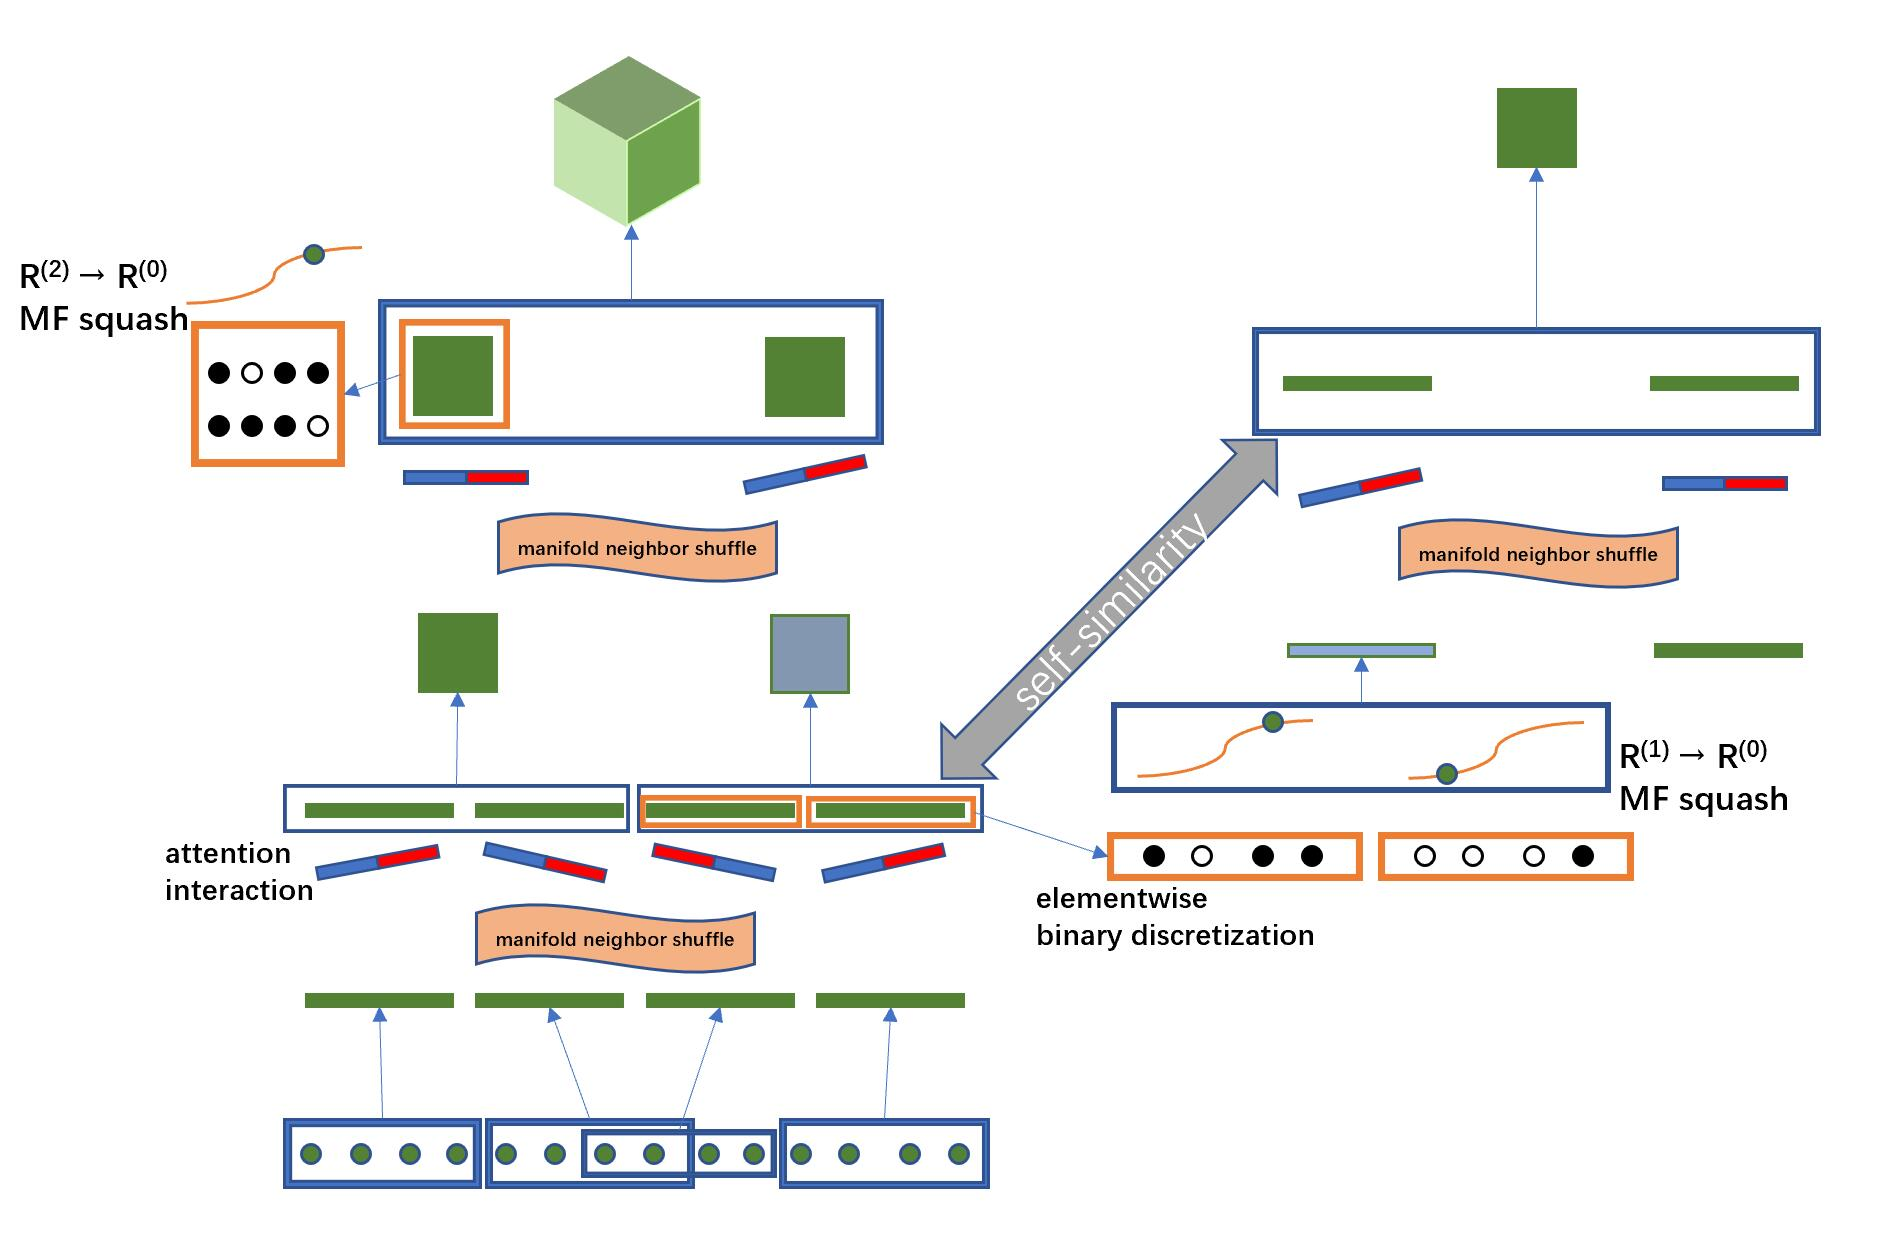
\includegraphics[width=1.0\linewidth]{fig/tower}}
  \caption{Boxes with arrows show aggregations. Overlapping aggregation is allowed in rank 0. Left attention tower is unsquashed ranks, versus right tower is squashed on rank 1, using mean field approximation.}\label{fig:tower}
\end{figure*}

\begin{figure*}[bth]
  \myfloatalign
  \subfloat[tanh-like function for $\beta \bar{n} J < 1$]
  {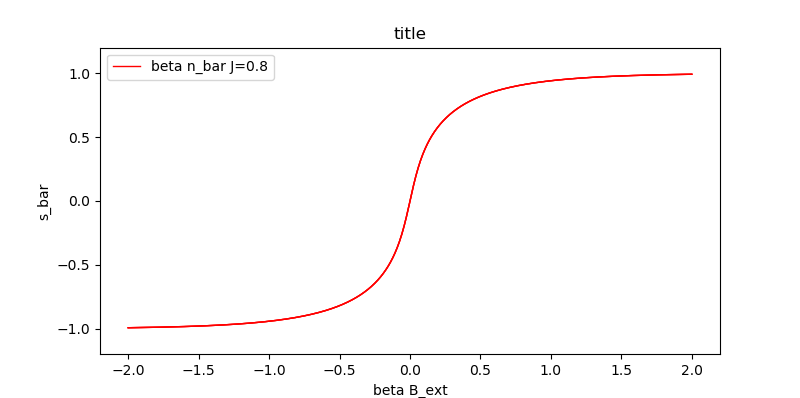
\includegraphics[width=.45\linewidth]{fig/transition_080}} \quad
  \subfloat[phase change for $\beta \bar{n} J > 1$]
  {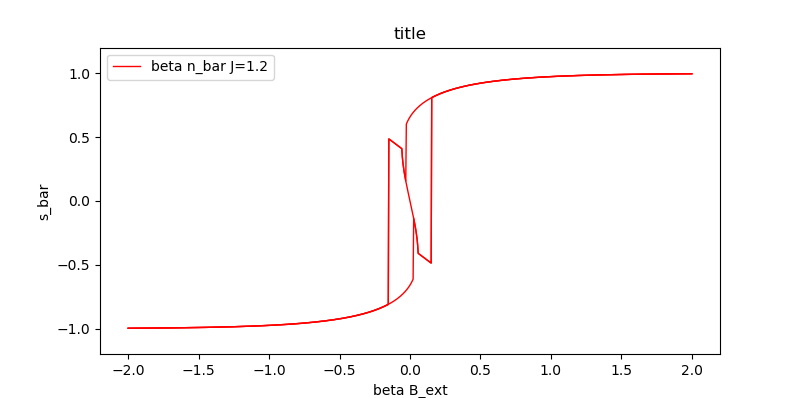
\includegraphics[width=.45\linewidth]{fig/transition_120}} \\

  \caption{non-linear activation function plotting $\mu$ against $\beta B_{ext}$}\label{fig:transCompare}
  \end{figure*}

\begin{multicols}{2}
  Plotting Eq\eqref{MF2} with $\beta |B_{ext}|$ on x-axis and mean-field $\mu$ on y-axis, there are two types of activation function obtained depending on whether the value of $\beta\bar{n} > 1.0$ or not. 
  Our experiment in (4.1) has proven the expected similarity between arriving signals will increase after training. 
  Therefore the number of similar signals exceeding threashold will also increase, causing the dipole-dipole interaction having more average number of similar neighbours, represented by $\bar{n}$. 

  There would be a point where the continuous activation function shown in Fig\ref{fig:transCompare}(a) becomes a discontinuous phase-transition allowed activation function shown in Fig\ref{fig:transCompare}(b) as $\bar{n}$ increases. 

  \subsection{Dissipative structure} 
  The most signifficant effect of phase transition is that small change in the external field can cause huge change in the induced mean field. 
  Tensors are nested in the hierachial structure and each tensor may exist in its critical state where phase change can be triggered with a small perturbation on the environment. 
  If there are a large proportion of tensors already in their critical state, then avalanche of phase transition would occure easily. 

  Energy dissipated into the surrounding environment in one switching cycle of mean field output, is proportional to the area enclosed by hysteresis in \ref{fig:transCompare}(b). 
  After the avalanche is stopped and the network reaches a new stable state, the entropy of the network is expected to be reduced. Dipole signals would interact in space-time diagram events with 
  more constructive interference and therefore having a lower entropy. As a result of second law of thermodynamics, the environment receives the dissipated energy and 
  the entropy of environment would increase to ensure the total entropy of universe $H_{universe}=H_{system}+H_{environment}$ to increase. 

  Sandpile model \\ \cite{PhysRevLett.59.381} is a good analogy towards the whole picture. High entropy input signals with energy provided by signal sources would 
  forward propagate through different distanced routes to be fed into the hierachial attention tensor. Different abstraction level (on different ranks) of tensors would estimate 
  their own mean field output, to complete the pooling process and then sending approximated signals to new destinations. Meanwhile route probabilities are updated by simple rule 
  described in Eq\ref{eq:update-rule}. This update enables the mean field attentions to have a lower entropy most of the time; also it doesn't require information back propagated from top-layer, 
  but only requires the nearby external magnetic field, so updating can be done locally. Because the local target field can change with time, it is possible that 
  within an attention tensor, phase change can produce discontinuous output, triggering phase change in other tensors connected with it after the signal travelling time. 
  An avalanche can propagate within a much larger region of brain just like the sandpile model. Self-organization is expected to be observed after avalanche so that the network system can maintain itself by comsuming 'negative entropy' \cite{schrodinger1962life}. 


\end{multicols}

\section{Conclusion}
\begin{multicols}{2}
  Self-attention mechanism has been proven successiful in rescent year transformer-based encoders. By realizing the physical interpretation of self-attention being signal interactions, 
  ising model becomes a viable choice of modelling a learning process. Despite the forces governing the interaction remain unknown, its physical property is assumed to be similar as magnetic force. 
  By fixing positions of signal sources and target region, then setting signal travel speed to be constant, space-time condition where an ising model interaction event takes place can be identified. 
  This brings the idea of travelling routes and constructive interference defined same as in optics. Training process is trying to make constructive interference among input and target signals at a specified position. 
  Once route probabilities are trained, no matter whether target signal is still present or not, constructive interference would retain, because the input signals would still interfere with each other. 

  A constructive interference also suggests the potential energy of system is minimized, therefore by ignoring the dipole-dipole energy, but keeping the dipole-target energy, an simplified energy-based goal is proposed. 
  Probabilities of routes with different travelling time are updated for each source-destination pair, in the aim of optimizing our goal. 

  Two experiments were designed. One did a 4-class MNIST classification, showing good few-shot performance, and it was immune to catastrophic forgetting. 
  It also confirmed the induction by target signal was effective, as the expected dipole-dipole similarity was highest in the correct target's position even if the target signal was absense. 
  The second experiment did a in-phase/out-of-phase periodic wave pattern binary classification, demonstrated time varying signals can also be learned using this interference idea. 

  A failed NLP task attempt lead to the reconsideration of using word vectors. A nested aggregation, mean field pooling and attention interaction mechanism is proposed. It brought the following features into our learner. 

  \begin{enumerate}
    \item It has a fractal structure, with self-similarity between different ranks and different scales.
    \item Mean field pooling lowers the number of updating routes towards the next destination if the tensor learner is relaying signals. This makes future calculations to be more efficient. 
    \item Mean field brings back the previously ignored dipole-dipole interaction. It allows the tensor learner to have a critical state. The constituent sub-ranked tensors can also have their own critical states. 
    \item Avalanche of phase transition can occure and propagate throughout the network system containing a large number of learners. Avalanche magnitude versus frequency graph may not obey the power law, because we know human brain is actively maintaing the brain's critical state \cite{brochini2016phase}. Therefore it is reasonable to assume that the stopping condition of training is to keep the tensors in network not too far from their critical states. 
    \item Non-linearity and discontinuity emerge as a consequence of phase transition. 
    \end{enumerate}
  
  All the evidences are pointing towards dissipative structure and edge of chaos. It would be interesting to study signal interference in such a complex system.
\end{multicols}

\bibliographystyle{acl_natbib}
\bibliography{reference}
\end{document}